\documentclass[12pt,a4paper]{report}
\usepackage[a4paper,left=2.9cm,right=2.9cm,top=2.6cm,bottom=2.6cm]{geometry}
\usepackage[T1]{fontenc}
\usepackage{mathptmx}
\usepackage{microtype}
\usepackage{graphicx}
\usepackage{amsmath,amssymb}
\usepackage{booktabs,array,tabularx}
\usepackage{enumitem}
\usepackage{float}
\usepackage[font=small]{caption}
\usepackage{titlesec}
\usepackage{xcolor}
\usepackage[hidelinks,pageanchor=false]{hyperref}

\setlist{itemsep=2pt,topsep=4pt}
\setlength{\parindent}{1.0cm}
\setlength{\parskip}{3pt}
\linespread{1.12}
\captionsetup{labelsep=colon}
\graphicspath{{fig/}}

% chapter and section styles close to the department template
\titleformat{\chapter}[display]{\normalfont\bfseries\centering}{\Large Chapter \thechapter}{14pt}{\Large\MakeUppercase}
\titlespacing*{\chapter}{0pt}{20pt}{30pt}
\titleformat{\section}{\normalfont\sffamily\Large\bfseries}{\thesection}{1em}{}
\titleformat{\subsection}{\normalfont\sffamily\large\bfseries}{\thesubsection}{1em}{}

\usepackage{soul}
\sethlcolor{yellow}
\newcommand{\todo}[1]{\hl{#1}}
\newcommand{\code}[1]{\texttt{#1}}
\newcommand{\pp}{\,pp}
\renewcommand{\bibname}{References}

\begin{document}

% ---------------------------------------------------------------- cover
\pagestyle{empty}
\begin{center}
\vspace*{1.6cm}
{\large\bfseries MAJOR PROJECT REPORT}\\[10pt]
on\\[14pt]
{\LARGE\bfseries Action Risk Calibrated Remediation:\\[4pt] A Benchmark and Graph Model for\\[4pt] Predicting the Blast Radius of Automated\\[4pt] Remediation in Microservices}\\[26pt]
Submitted in partial fulfilment for the Award of Degree of\\[20pt]
{\large\bfseries BACHELOR OF ENGINEERING}\\[6pt]
{\large\bfseries IN}\\[6pt]
{\large\bfseries INFORMATION TECHNOLOGY}\\[24pt]
{\bfseries BY}\\[8pt]
ABHISHEK KUMAR SINGH (160123737094)\\
LAKSH JAIN (160123737120)\\
YOGESH CHOUDHARY (160123737125)\\[22pt]
Under the guidance of\\[8pt]
{\bfseries Dr. RAMAKRISHNA KOLIKIPOGU}\\
Professor\\[24pt]
{\bfseries DEPARTMENT OF INFORMATION TECHNOLOGY}\\[4pt]
{\bfseries CHAITANYA BHARATHI INSTITUTE OF TECHNOLOGY (A)}\\[4pt]
{\small (Affiliated to Osmania University; Accredited by NBA (AICTE) and NAAC (UGC),\\
ISO Certified 9001:2015), Kokapet (V), Gandipet (M), Hyderabad -- 500 075}\\
{\small Website: \texttt{https://www.cbit.ac.in}}\\[14pt]
2026--2027
\end{center}
\newpage

% ---------------------------------------------------------------- front matter
\pagenumbering{roman}
\pagestyle{plain}

\chapter*{Certificate}
\thispagestyle{plain}
\vspace{-6pt}
This is to certify that the major project report entitled \textquotedblleft Action Risk Calibrated Remediation: A Benchmark and Graph Model for Predicting the Blast Radius of Automated Remediation in Microservices\textquotedblright{} submitted to Chaitanya Bharathi Institute of Technology, in partial fulfilment of the requirements for the award of degree of B.E. (Information Technology) during the academic year 2026--27 is a record of original work carried out by Abhishek Kumar Singh (160123737094), Laksh Jain (160123737120) and Yogesh Choudhary (160123737125) during the period of study in the Department of Information Technology, CBIT, Hyderabad.

\vspace{3.2cm}
\noindent
\begin{tabular}{@{}p{7.2cm}p{7cm}@{}}
\textbf{Project Guide} & \textbf{Head of the Department}\\
Dr. Ramakrishna Kolikipogu & \todo{Dr. M. Venu Gopalachari}\\
Professor, IT Dept. & Professor, IT Dept.\\
CBIT, Hyderabad. & CBIT, Hyderabad.
\end{tabular}
\newpage

\chapter*{Abstract}
\addcontentsline{toc}{chapter}{Abstract}
Automated incident-response tools for microservice systems restart, scale or drain a service to restore normal operation, and they decide whether to act by how confident they are about the root cause. Confidence says nothing about what the chosen action will cost: the action changes the traffic and load of the services around its target, and services that were healthy can start to fail or slow down. This report presents ARC (Action Risk Calibrated Remediation), a benchmark and a graph model that predict, before an action is applied, how much each service will be damaged by it. Damage is measured as the rise in the share of a service's requests that fail or become slow, over the 180 seconds after the action. We built a Kubernetes testbed with the Train Ticket application, injected faults, applied six remediation actions and recorded 1,795 controlled incidents, each labelled per service from exact request counters. A three-layer message-passing network over the service call graph, trained on the state of every service in the 60 seconds before the action, cuts the prediction error roughly in half against the best baseline in every test: 1.98 against 3.86 percentage points on new incidents of the same system, 2.86 against 3.91 on an unseen system, and 1.86 against 2.61 on an unseen fault. It names the most damaged service in 78\% of incidents, scores all six candidate actions in about 25 ms, and drives a block, ask or allow gate that blocks 1.6\% of safe actions and detects 84\% of harmful ones. The model does not yet predict faults of a new kind, such as a four-times traffic surge, and these limits are reported. The dataset is prepared for open release.

\vspace{6pt}
\noindent\textbf{Index Terms}---AIOps, automated remediation, microservices, blast radius, graph neural networks, fault injection, benchmark dataset.
\newpage

\tableofcontents
\newpage
\listoffigures
\addcontentsline{toc}{chapter}{List of Figures}
\newpage
\listoftables
\addcontentsline{toc}{chapter}{List of Tables}
\clearpage

% ---------------------------------------------------------------- body
\pagenumbering{arabic}

\chapter{Introduction}
\section{Overview}
Modern online services are built from many small programs called microservices. A user request, for example booking a train ticket, passes through a chain of services, and each one calls others. The map of which service calls which is the \emph{call graph}. When one service fails or slows down, tools that watch the system, often called AIOps tools, try to repair it automatically. The common repairs are to restart the service, to start more copies of it, to give it more CPU, or to take it out of rotation (drain it). Recent systems use large language models or learned diagnosers to find the root cause of the incident and to choose the repair~[12],[4].

These tools decide to act on how confident they are about the diagnosis. That confidence says nothing about what the repair will cost. Restarting one service stops the traffic it was serving; the services that call it see errors, and the services it calls suddenly receive fewer requests. A service that was healthy before the repair can therefore fail or slow down because of it. In an experiment on the Train Ticket application, restarting a single service after a network delay raised the share of failed or slow requests in several other services (Chapter~4).

This project addresses the missing step: predicting, before an action is applied, how much damage it will cause to each service. We call the system \textbf{ARC} (Action Risk Calibrated Remediation). ARC reads the recent state of every service, the call graph and the candidate action, and answers in milliseconds. This report describes the testbed we built, the dataset of 1,795 controlled incidents we recorded and labelled, the graph model that predicts the damage, the explanation and decision layers on top of it, and the evaluation.

\noindent This project can be used to:
\begin{itemize}
\item \textbf{Check an action before it runs:} an agent or an on-call engineer asks ARC what a restart, scale-up or drain would do to every service, and receives a block, ask or allow recommendation.
\item \textbf{Choose the safest repair:} the same incident is scored for each of six candidate actions, and the one with the lowest predicted damage is suggested.
\item \textbf{Explain the blast radius:} ARC shows which services will be hit, by how much, and through which call path.
\item \textbf{Benchmark new methods:} the released dataset gives researchers per-service damage labels and raw telemetry, which no existing public dataset records.
\end{itemize}

\section{Problem Definition}
Autonomous remediation tools do not predict the consequences of the actions they choose. The problem is to predict this damage before the action is applied. Given the state $s$ of every service during the 60~seconds before the action, the call graph $G$, and a candidate action $a$ with its target service, the model $f$ must output for every service $i$ the predicted rise $\hat{y}_i$ of the share of its requests that fail or become slow during the next 180~seconds:
\[
f(G, s, a) \rightarrow \hat{y} = (\hat{y}_1, \ldots, \hat{y}_n),
\]
where $n$ is the number of services and $\hat{y}_i$ is measured in percentage points. The prediction must not use knowledge of the fault, must be fast enough for an agent to ask before every action, and must still hold on a system, a load and a fault type it was not trained on.

\section{Aim of the Project}
To develop and evaluate a learned model that predicts the per-service damage of automated remediation actions before they are applied, and to release a measured dataset that makes such models possible to build and compare. The objectives are:
\begin{enumerate}
\item to build a repeatable testbed that injects faults, applies remediation actions and records telemetry unattended;
\item to define a damage label that is measured from exact request counts and is robust to the choice of latency threshold;
\item to record a large, balanced dataset of incidents with all six actions applied to each fault condition;
\item to train a graph model and compare it with simple, tree-based and LLM-based baselines on new incidents, a new system, a new fault, a higher load and repeated incidents;
\item to add an explanation of the blast radius, a ranking of actions and a decision gate; and
\item to report the limits of the approach honestly, including the cases it does not predict.
\end{enumerate}

% ----------------------------------------------------------------
\chapter{Literature Survey}
This chapter reviews the work closest to ours. Each entry gives the title, authors and venue, what the work does, and what it leaves open for this project. The works are grouped in our references at the end of the report.

\section{Paper 1}
\noindent\textbf{Title:} TAMO: Fine-Grained Root Cause Analysis via Tool-Assisted LLM Agent with Multi-Modality Observation Data in Cloud-Native Systems\\
\textbf{Authors:} X. Zhang, Q. Wang, M. Li, Y. Yuan, M. Xiao, F. Zhuang, D. Yu\\
\textbf{Publisher:} IEEE Transactions on Services Computing, 2025 [12]\\
\textbf{Description:} The paper uses a tool-assisted large language model agent that reads metrics, logs and traces to localise the root cause of an incident and to classify the fault. It is the base paper of this project.\\
\textbf{Gaps:} It finds what failed but does not predict what a repair will do to the other services. Per-service damage of remediation is outside its scope.

\section{Paper 2}
\noindent\textbf{Title:} RCAEval: A Benchmark for Root Cause Analysis of Microservice Systems with Telemetry Data\\
\textbf{Authors:} L. Pham, H. Zhang, H. Ha, F. Salim, X. Zhang\\
\textbf{Publisher:} WWW 2025; arXiv:2412.17015 [13]\\
\textbf{Description:} A benchmark of 735 failure cases from three microservice systems, with 15 baseline root-cause methods, covering metrics, logs and traces.\\
\textbf{Gaps:} It records faults and their root causes, not the consequences of repairs. It cannot be used to learn what an action does to the neighbouring services.

\section{Paper 3}
\noindent\textbf{Title:} MicroRemed: Benchmarking LLMs in Microservices Remediation\\
\textbf{Authors:} L. Zhang et al.\\
\textbf{Publisher:} arXiv:2511.01166, 2025 [4]\\
\textbf{Description:} A benchmark for language models that write executable remediation playbooks from a diagnosis, together with a multi-agent method (ThinkRemed).\\
\textbf{Gaps:} The focus is generating repairs. It does not predict the per-service impact of a repair before it is run.

\section{Paper 4}
\noindent\textbf{Title:} Safe Remediation as Risk-Constrained Intervention Decision in Microservice Systems\\
\textbf{Authors:} C. Dai, Z. Yan, C. Lei, Q. Li, L. Zhang\\
\textbf{Publisher:} arXiv:2607.20005, 2026 [1]\\
\textbf{Description:} Safe remediation is treated as a risk-constrained decision. Risk combines blast radius, reversibility and uncertainty, and a human-in-the-loop gate approves risky actions. The authors report 1,664 events and 8,320 decision records on Train Ticket, a 39\% lower false-remediation rate and 17\% fewer on-call escalations.\\
\textbf{Gaps:} Labels are per decision (resolved, partial or false remediation), not the damage to each service. We found no public code or data.

\section{Paper 5}
\noindent\textbf{Title:} Can AI Remediate Backend Failures Safely? GuardedAct with Blast-Radius-Aware Sandboxing\\
\textbf{Authors:} W. Cai et al.\\
\textbf{Publisher:} arXiv:2609.11264, 2026 [2]\\
\textbf{Description:} A language model proposes actions, a digital-twin sandbox estimates their blast radius, and a rollback-confidence gate decides. On DeathStarBench the authors report an 87.4\% recovery rate and collateral damage falling from 25.6\% to 5.2\%, with about 8 s of added recovery time.\\
\textbf{Gaps:} Simulation adds delay to every decision. ARC targets a fast learned prediction (about 4 ms per action) rather than a sandbox run.

\section{Paper 6}
\noindent\textbf{Title:} Autonomous Incident Resolution at Hyperscale: An Agentic AI Architecture for Network Operations\\
\textbf{Authors:} A. Malik\\
\textbf{Publisher:} arXiv:2606.09122, 2026 [6]\\
\textbf{Description:} A multi-agent architecture with graduated autonomy, deployed at a major cloud provider, in which more than 90\% of common incidents are resolved autonomously.\\
\textbf{Gaps:} No model of the consequences of individual actions on other components is reported.

\section{Paper 7}
\noindent\textbf{Title:} AIOpsLab: A Holistic Framework to Evaluate AI Agents for Enabling Autonomous Clouds\\
\textbf{Authors:} Y. Chen et al.\\
\textbf{Publisher:} arXiv:2501.06706, 2025 [9]\\
\textbf{Description:} A framework for evaluating AI agents on cloud operations tasks, with injected faults and an agent--cloud interface.\\
\textbf{Gaps:} It scores whether an agent solves the task. It does not measure, per service, how much collateral damage the agent's actions cause.

\section{Summary of the Gap}
Table~\ref{tab:gap} summarises what each line of work provides. None of them offers a learned, per-service prediction of the damage of a repair, trained on a released dataset of measured repair outcomes.

\begin{table}[H]
\centering
\caption{What related work provides and what ARC adds.}
\label{tab:gap}
\small
\begin{tabularx}{\textwidth}{>{\raggedright\arraybackslash}p{3.1cm}XXXX}
\toprule
Work & Finds root cause & Generates repair & Estimates repair risk & Per-service damage prediction \\
\midrule
TAMO [12] & yes & -- & -- & -- \\
RCAEval [13] & dataset only & -- & -- & -- \\
MicroRemed [4] & -- & yes & -- & -- \\
Dai et al. [1] & -- & -- & per decision & -- \\
GuardedAct [2] & -- & yes & sandbox (slow) & estimated in sandbox \\
\textbf{ARC (this work)} & -- & -- & learned, 4 ms per action & \textbf{yes, with released data} \\
\bottomrule
\end{tabularx}
\end{table}

% ----------------------------------------------------------------
\chapter{System Requirement Specification}
\section{Functional Requirements}
\begin{enumerate}
\item The system must run a controlled incident unattended: check that the cluster is healthy, record a baseline, inject a fault, wait, apply one remediation action, measure, and store the result.
\item The system must support nine fault types (no fault, pod-kill, hung pod, network delay, packet loss, CPU squeeze, database delay, call cut and load surge) and six actions (no-op, restart-pod, rollout-restart, scale-up, cpu-bump and drain).
\item The system must plan campaigns in advance in blocks of seven episodes (one fault condition, one episode per action, no-op twice) so that action effects can be compared within the same kind of incident.
\item The system must record, for every episode, per-service request rates, errors, latency percentiles, CPU, memory and readiness every 5 seconds, the call graph with its failed calls, and every request the load generator sent.
\item The system must compute, for every service, the share of bad requests before and after the action, and the damage labels (mean, peak and recovery time), from exact request counters.
\item The system must calibrate the latency bar that defines a slow request on healthy episodes only, and check it on healthy episodes that were not used to fit it.
\item The system must flag episodes that were already saturated before the action, episodes with a machine stall, and services with too few requests to score.
\item The model must predict, for every service, the damage of a candidate action using only information available before the action.
\item The system must score all six candidate actions for one incident and recommend the one with the lowest predicted net damage.
\item The system must explain the blast radius: which services are hit, by how much, and through which call path from the target.
\item The system must return a block, ask or allow decision, using the predicted damage and the disagreement between model copies.
\item The system must clean up after every episode (faults, partitions, resized pods, scaled replicas) and stop safely after repeated failures.
\item The system must export every episode in an open format and provide a loader and checksums so that the dataset can be reused.
\end{enumerate}

\section{Non-Functional Requirements}
\subsection{Speed and Memory Requirements}
A prediction must be fast enough for an agent to ask before every action. The graph model scores one action in about 4~ms and all six candidate actions in about 25~ms on a CPU. The complete tool, with five model copies, the tree blend and the explanation, takes about 350~ms and has not been optimised. Data collection is slower by design: one episode takes about 9 minutes and a campaign of several hundred episodes runs for days. The model itself is small (hidden vectors of 64 numbers) and needs no GPU for prediction.

\subsection{Usability Requirements}
An engineer or an agent must be able to ask ARC about an incident with one command and receive a short, readable answer: the decision, the predicted damage per service and the call chain behind it. A live viewer shows the state of the cluster and the call graph so that a campaign can be supervised. The released dataset has a datasheet, a schema description and a loader so that it can be used without knowing the testbed.

\subsection{Reliability and Reproducibility Requirements}
Campaigns must run unattended for days. The runner therefore checks the health of the cluster before every episode, repeats or discards an episode that fails its checks, stops after two failures in a row, and guards disk space. Plans are fixed before a campaign starts and every decision that changes the method is written in a decision log.

\section{Software Requirements}
\begin{itemize}
\item \textbf{Operating System:} Linux for the lab machine; Windows 11 with WSL2 for development.
\item \textbf{Containers and cluster:} Docker, Kubernetes 1.34 (kind).
\item \textbf{Applications under test:} Train Ticket (20 to 25 services) and Online Boutique (11 services plus a cache).
\item \textbf{Fault injection:} Chaos Mesh 2.6.3, with in-place pod resizing for the CPU squeeze.
\item \textbf{Telemetry:} OpenTelemetry Collector (span metrics and service graph), Prometheus (5 s resolution), cAdvisor, kube-state-metrics, Grafana.
\item \textbf{Languages and libraries:} Python 3, NumPy, PyTorch, shell scripts.
\item \textbf{Version control and release:} Git and GitHub for code; Zenodo and Hugging Face for the dataset.
\end{itemize}

\section{Hardware Requirements}
\begin{itemize}
\item \textbf{Data collection:} one workstation with an Intel Core i9-13900 processor (20 cores) and 32~GB of memory runs the whole cluster, the load generator and the telemetry stack; tens of gigabytes of free disk space for container images and metrics.
\item \textbf{Modelling:} a laptop is enough; training and prediction run on the CPU.
\item \textbf{Prediction at run time:} a single CPU core.
\end{itemize}

% ----------------------------------------------------------------
\chapter{Methodology / Proposed System}
\section{System Architecture / System Design}
ARC is organised in five layers (Figure~\ref{fig:arch}). At the bottom, a Kubernetes testbed runs the application under test and an open-loop load generator that keeps the offered load constant even when the system slows down. Above it, the experiment harness injects faults, applies remediation actions and plans campaigns. The data pipeline turns the telemetry of each episode into features and damage labels. The ARC layer holds the graph damage model, the dynamic model, the blast-radius explainer and the decision gate. At the top, an interface lets an agent or an engineer ask about a candidate action before it is executed.

\begin{figure}[H]
\centering
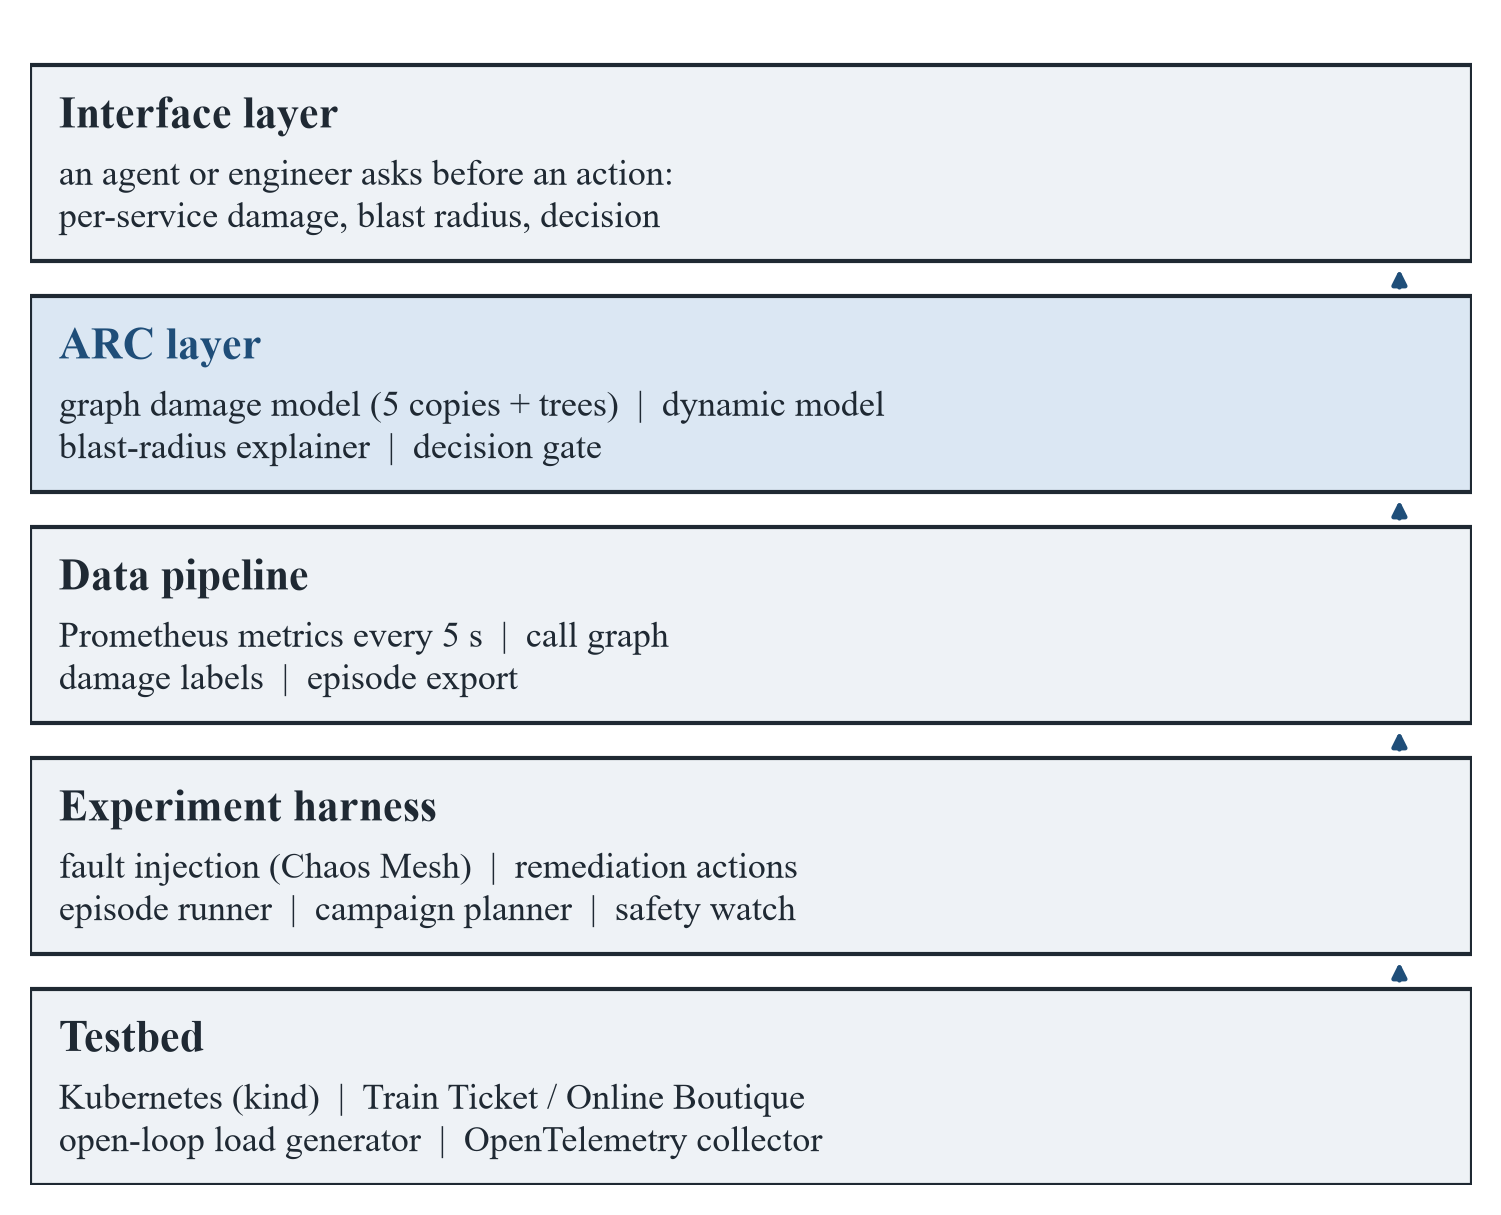
\includegraphics[width=0.82\textwidth]{arch.png}
\caption{Layered architecture of ARC.}
\label{fig:arch}
\end{figure}

Figure~\ref{fig:flow} shows the two flows through this architecture. In the data-collection flow (A) one episode is recorded: the cluster is checked, a 120 s baseline is taken, a fault is injected, the system waits 60 to 300 s, the state of the last 60 s is snapshotted, one random action is applied, and the next 180 s are measured and labelled. Everything the model uses is measured before the action; the label is measured after it. In the decision flow (B) the model reads the same pre-action state and the call graph and scores a candidate action; the damage per service becomes a blast-radius explanation and a decision.

\begin{figure}[H]
\centering
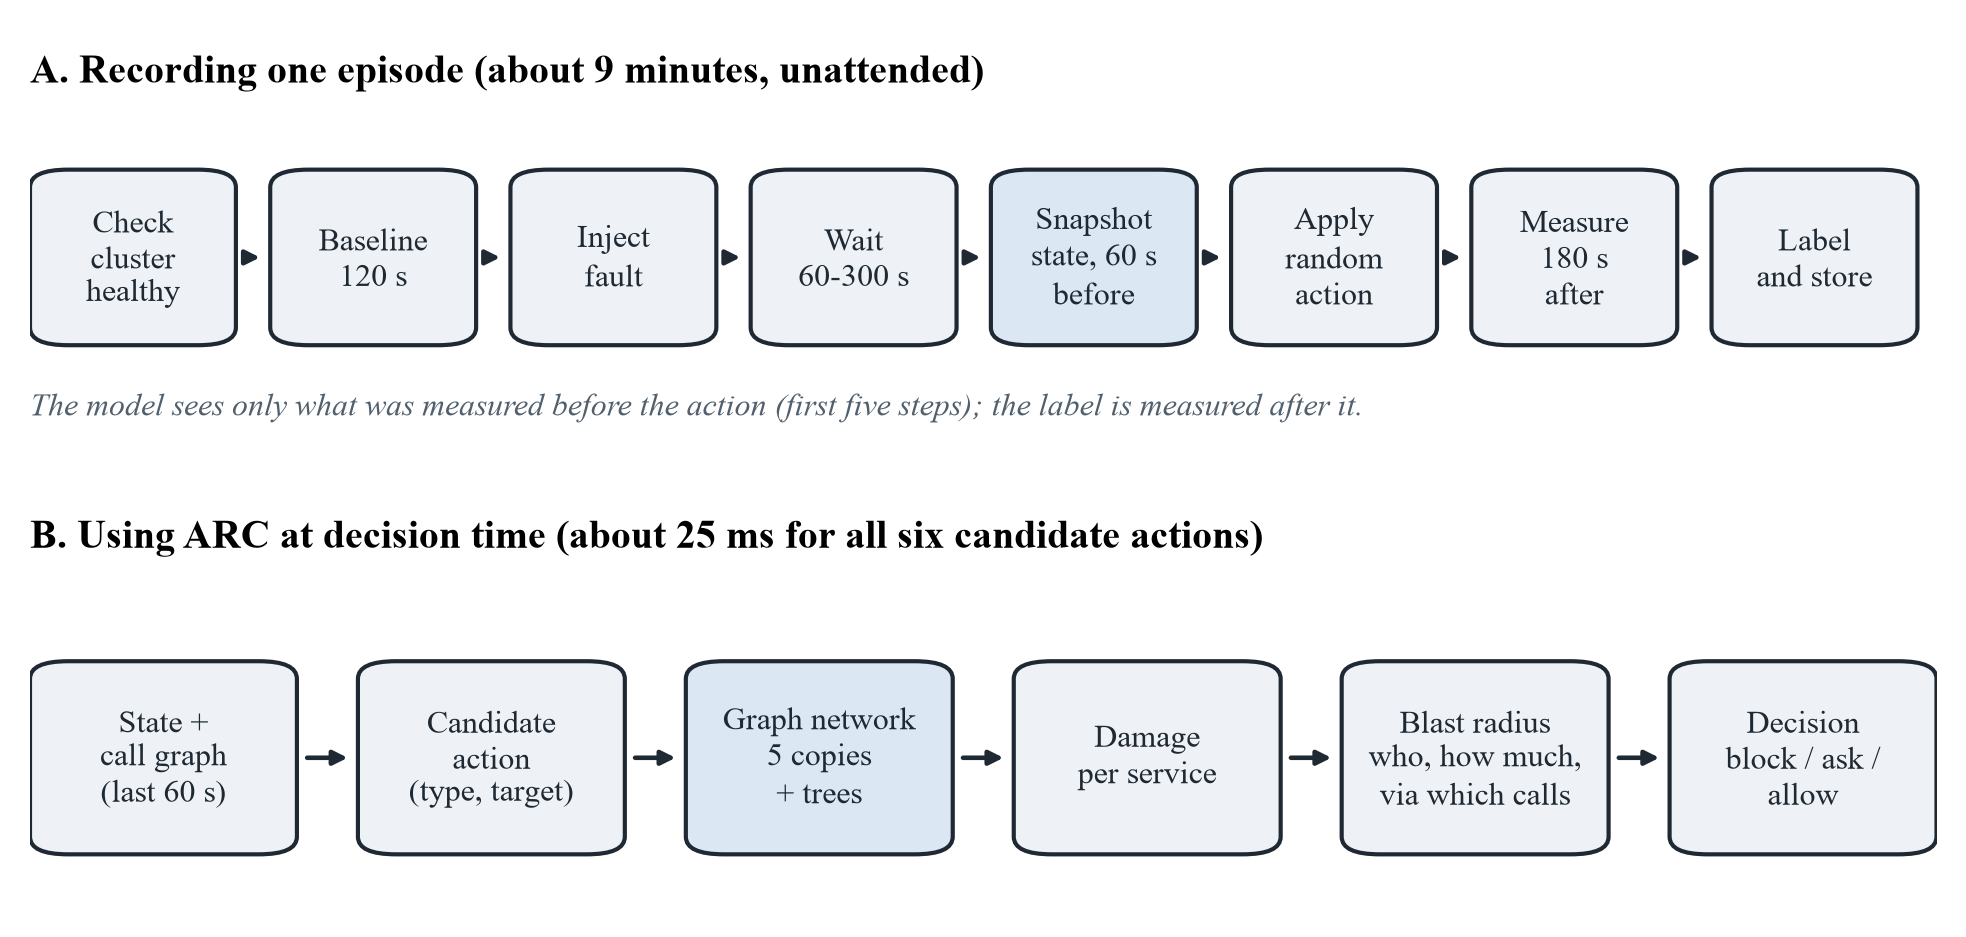
\includegraphics[width=\textwidth]{flow.png}
\caption{Flow chart of the proposed system: (A) recording one episode and (B) using ARC at decision time.}
\label{fig:flow}
\end{figure}

\section{Testbed and Data Collection}
\subsection{Application and infrastructure}
The main application is Train Ticket~[20], a ticket-booking system of 20 services in its core form and 25 in its wide form, written mostly in Java. It runs on Kubernetes 1.34 inside kind on one workstation. OpenTelemetry spans reach Prometheus through the collector, which produces per-service request rates, latency histograms and the service call graph every 5 seconds; cAdvisor and kube-state-metrics supply CPU, memory and readiness. Chaos Mesh~[22] injects the faults. A load generator sends nine kinds of user requests (search, orders, booking, payment, cancel and collection flows) at 4 or 8 requests per second with Poisson arrivals.

\subsection{Faults and actions}
Each episode injects one fault and applies one action 60 to 300 seconds later. Table~\ref{tab:fa} lists the nine fault types and six actions and how often each occurs in the dataset.

\begin{table}[H]
\centering
\caption{Faults and actions in the dataset (episodes).}
\label{tab:fa}
\small
\begin{tabular}{@{}lr@{\hspace{1.2cm}}lr@{}}
\toprule
Fault & Episodes & Action & Episodes \\
\midrule
none & 273 & no-op (control) & 512 \\
packet loss & 467 & restart-pod & 259 \\
network delay & 434 & rollout-restart & 258 \\
pod-kill & 273 & drain & 258 \\
hung pod & 119 & scale-up & 255 \\
CPU squeeze & 61 & cpu-bump & 253 \\
database delay & 63 & & \\
call cut & 63 & & \\
load surge & 42 & & \\
\bottomrule
\end{tabular}
\end{table}

The actions are: \textbf{restart-pod} (delete the pod so that a new one starts), \textbf{rollout-restart} (replace the pod through the deployment), \textbf{scale-up} (add a second copy), \textbf{cpu-bump} (raise the CPU limit in place), \textbf{drain} (take the instance out of rotation without stopping it) and \textbf{no-op} (do nothing; the control). Because the no-op is applied to every fault condition, the damage of an action can be separated from the damage of the fault itself.

\subsection{Campaign design}
A campaign is planned before it runs. It is cut into blocks of seven episodes that share one fault condition: one episode per action, and the no-op twice. Blocks never straddle the split between training and test data. The campaign runs unattended, 6 to 7 episodes per hour, with a health check before each episode, an automatic repeat of an episode that fails, a disk guard and a safety watch. The six parts of the dataset were recorded between 17 and 26 October 2026 on one Intel i9-13900 workstation with 32~GB of memory.

\section{Damage Label}
\subsection{Bad requests and measurement windows}
A request is \emph{bad} if it fails or takes longer than a latency bar. We use three bars: a per-operation bar calibrated on healthy episodes (99th percentile of healthy latency, with a floor of 100~ms), and fixed bars of 500~ms and 1~s. The \emph{bad-request share} of a service in a window is the number of its bad requests divided by all its requests.

For every action, two windows are used (Figure~\ref{fig:windows}). The baseline window $B$ is the 60~s before the action. The measurement window $M$ starts 5~s after the action, lasts 180~s and is divided into six blocks $b_1,\dots,b_6$ of 30~s.

\begin{figure}[H]
\centering
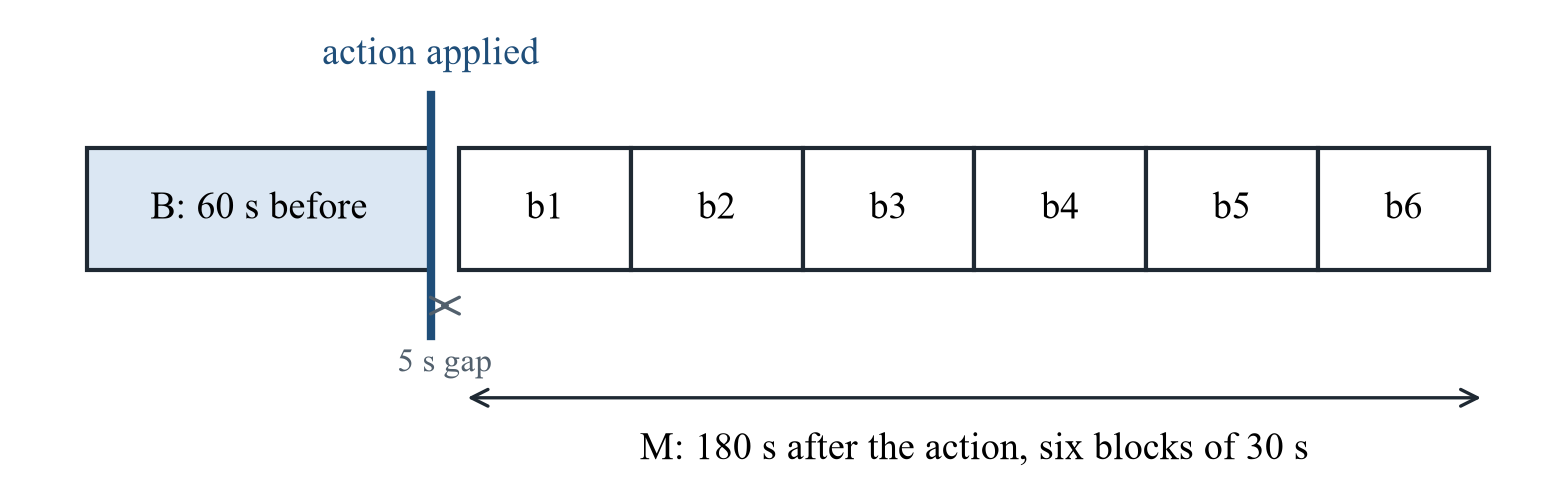
\includegraphics[width=0.95\textwidth]{windows.png}
\caption{Baseline window $B$ and measurement window $M$ around the action.}
\label{fig:windows}
\end{figure}

\subsection{Damage measures}
The \emph{mean damage} of service $i$ is the change of its bad-request share between the two windows:
\begin{equation}
y_i^{\mathrm{mean}} = p_i^{M} - p_i^{B}, \qquad p = \frac{\text{bad requests}}{\text{all requests}}.
\end{equation}
For example, a service that went from 2\% bad requests to 7\% has a mean damage of 5 percentage points (pp). A block with few requests could show exactly 0\% or 100\%, so for the per-block shares half a request is added to the counts:
\begin{equation}
\tilde{p}_{ib} = \frac{\mathrm{bad}_{ib} + 0.5}{n_{ib} + 1}.
\end{equation}
The \emph{peak damage} is the largest increase in any 30-second block, which exposes short, sharp harm that an average hides:
\begin{equation}
y_i^{\mathrm{peak}} = \max_{b=1,\ldots,6}\ \tilde{p}_{ib} - \tilde{p}_i^{B}.
\end{equation}
The \emph{net effect} of an action is the sum of the mean damage over the services with enough traffic, that is at least 30 requests in both windows:
\begin{equation}
\mathrm{net}(a) = \sum_{i \in E} y_i^{\mathrm{mean}}, \qquad E = \{\, i : n_i^{B} \geq 30 \ \text{and}\ n_i^{M} \geq 30 \,\}.
\end{equation}
The net effect gives one score per action, which is what we use to compare actions. The labels also include the time a service takes to return to its baseline.

\subsection{Quality rules}
A service is scored only with 30 or more requests before and after the action. An episode in which at least 80\% of user requests were already bad before the action is flagged as saturated and analysed separately. An episode in which more than a quarter of the measurement window was lost to a machine stall is flagged as stalled. Every incident is repeated across all six actions. The latency bar is calibrated only on healthy no-op episodes: for Train Ticket it was fitted on 12 episodes and checked on 8 that were not used for fitting.

\section{The ARC Dataset}
Dataset v1.0 contains 1,795 campaign episodes in one table with a column that names the part, plus 80 healthy calibration episodes that are used only to fit the latency bars (Table~\ref{tab:parts}). Of the 37,790 labelled (episode, service) rows, 28,769 have enough requests to be scored. The dataset also records 4,696,050 individual user requests.

\begin{table}[H]
\centering
\caption{Parts of dataset v1.0.}
\label{tab:parts}
\small
\begin{tabular}{@{}lrllp{5.2cm}@{}}
\toprule
Part & Episodes & Services & Load & Faults \\
\midrule
batch 1 & 701 & 20 & 4 req/s & none, pod-kill, delay, loss, CPU squeeze \\
wide1 & 500 & 25 & 4 req/s & none, pod-kill, hung pod, delay, loss \\
wide1-db & 126 & 25 & 4 req/s & none, pod-kill, database delay \\
wide2 & 301 & 25 & 8 req/s & none, pod-kill, hung pod, delay, loss \\
repeat test & 20 & 25 & 8 req/s & 4 recipes repeated 5 times \\
held-out & 147 & 25 & 8 req/s & none, pod-kill, call cut (3 links), load surge (3x, 4x) \\
\bottomrule
\end{tabular}
\end{table}

For every episode the raw files are kept: per-service series every 5~s, the call graph with failed calls, exact request and latency-bucket counters, every request the load generator sent, Kubernetes events, the labels and the episode metadata. Any label can therefore be recomputed with another latency bar. The package has a datasheet, a schema description and a loader, checksums for every file, the licences (CC BY 4.0 for the data, MIT for the code), and host names and user paths were removed from the released files. It is prepared for release on Zenodo and Hugging Face.

\section{Damage Model}
\subsection{Input features}
Each service is described by 25 numbers: 13 state values measured in the 60~s before the action, a role code and the action type. The 13 state values are the request rate relative to the service's own healthy baseline, the error share, the 50th, 95th and 99th percentile latency relative to baseline, CPU use as a fraction of the limit, the share of CPU periods throttled, memory relative to baseline, whether the pod was ever not ready, the bad-request share before the action, an indicator that the service is the action target, and the shares of failed incoming and outgoing calls. All are relative to the service's own healthy level or bounded, so they mean the same on every machine, and the fault itself is never an input. The role code states the relation of the service to the action target: target, direct caller, multi-hop caller, callee or unrelated. The action type is one of the six actions.

\subsection{Graph network}
A service's damage depends on its callers and callees, so the model works on the call graph. Each service starts from an embedding of its features $x_i$, role $r_i$ and the action $a$:
\begin{equation}
h_i^{(0)} = \mathrm{ReLU}\big(W_0\,[x_i,\ r_i,\ a]\big),
\end{equation}
a hidden vector of 64 numbers. Three message-passing layers follow (Figure~\ref{fig:mp}). In each layer a service combines its own state with the mean state of its callers and the mean state of its callees, using separate weights for the two directions, and keeps its own state through a residual connection:
\begin{equation}
h_i^{(l+1)} = h_i^{(l)} + \mathrm{ReLU}\Big( W_s\, h_i^{(l)} + W_c\, \overline{h^{(l)}_{\mathrm{callers}(i)}} + W_e\, \overline{h^{(l)}_{\mathrm{callees}(i)}} \Big), \quad l = 0,1,2.
\end{equation}
A small head maps the final vector to the predicted damage of service $i$.

\begin{figure}[H]
\centering
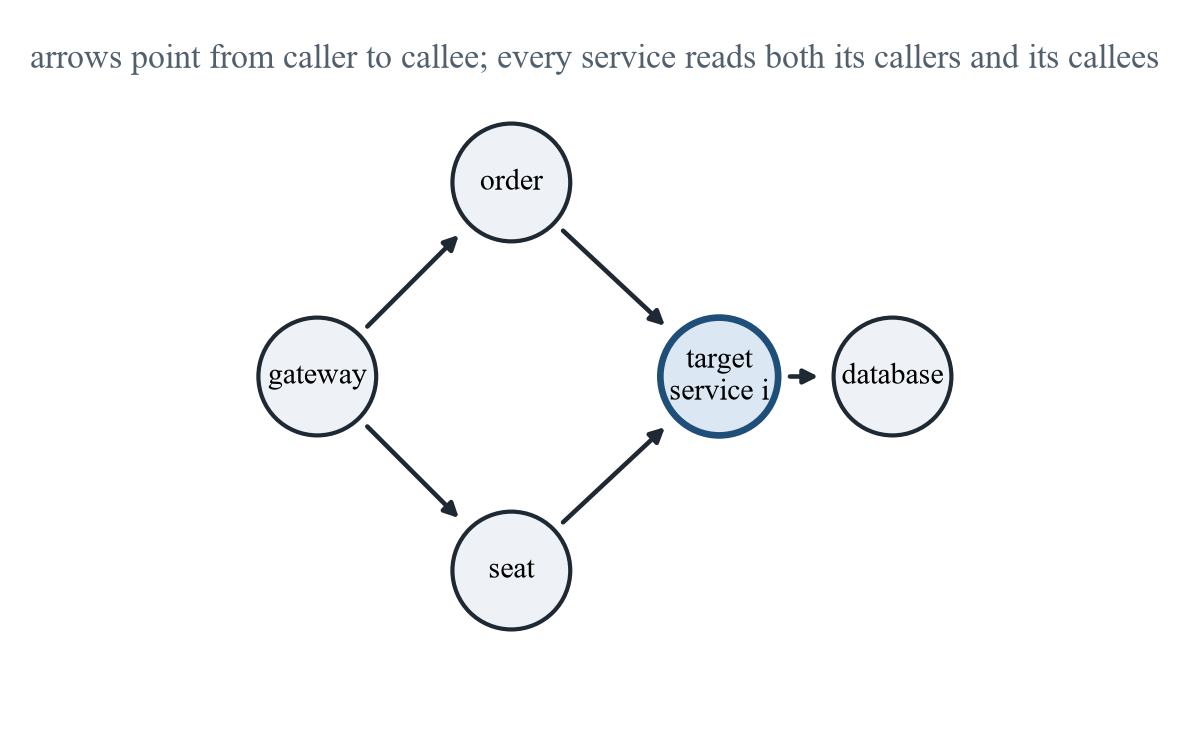
\includegraphics[width=0.78\textwidth]{mp.png}
\caption{Message passing: a service reads the state of its callers and of its callees.}
\label{fig:mp}
\end{figure}

\subsection{Training and final prediction}
The network is trained with the L1 loss (mean absolute error) and the Adam optimiser with early stopping on a validation set made of whole blocks. Five random seeds give five model copies. The final prediction is a weighted ensemble of the graph model and a tree model:
\begin{equation}
\hat{y} = 0.9\,\hat{y}^{\mathrm{GNN}} + 0.1\,\hat{y}^{\mathrm{trees}},
\end{equation}
where $\hat{y}^{\mathrm{GNN}}$ is the mean of the five copies. The spread of the five copies is used as an uncertainty estimate.

\section{Blast Radius, Action Choice and Decision Gate}
\subsection{Blast radius}
Damage spreads through the call graph. Let $d_i(k)$ be the extra bad-request share of service $i$, $k$ steps of 15~s after the action. A linear model fitted on the recorded trajectories describes how it moves:
\begin{equation}
d_i(k{+}1) = a\, d_i(k) + w_{dn}\, \overline{d_{\mathrm{callees}(i)}(k)} + w_{up}\, \overline{d_{\mathrm{callers}(i)}(k)} + g\, d_i(k_a) + u[a, \mathrm{role}_i, k - k_a].
\end{equation}
The fit says that a service keeps most of its own damage ($a = 0.84$) and is pulled by the damage of the services it calls ($w_{dn} = 0.17$) about nine times more than by the services that call it ($w_{up} = 0.02$). The term $g$ is the fault still present at the action, and $u$ is the action's own effect for each role and step. The chain shown to the user is the shortest call path from the target to each service that is hit.

\subsection{Choosing an action}
The same incident is scored six times, once for each candidate action, and the safest action is the one with the lowest predicted net effect:
\begin{equation}
a^{*} = \arg\min_{a \in \mathcal{A}} \widehat{\mathrm{net}}(a), \qquad |\mathcal{A}| = 6.
\end{equation}

\subsection{Decision gate}
The gate turns the predicted net effect and the disagreement of the five copies, $\sigma(a)$, into a decision:
\begin{equation}
\mathrm{decision}(a) =
\begin{cases}
\text{block} & \text{if } \widehat{\mathrm{net}}(a) \geq 20,\\
\text{ask a human} & \text{if } \sigma(a) \geq \sigma_0,\\
\text{allow} & \text{otherwise.}
\end{cases}
\end{equation}
Twenty points of net damage is the blocking threshold. The disagreement threshold $\sigma_0$ is the 90th percentile of the copies' spread on training actions that would not be blocked, so it is set on training data only.

\section{Experimental Setup and Evaluation Protocol}
\subsection{Baselines}
ARC is compared with: \textbf{no damage} (predict zero), a \textbf{runbook average} (the average damage seen for the same action), a \textbf{role rule} (the average damage for the service's role relative to the target), a \textbf{dependency map} (damage assigned to services connected to the target in the call graph), \textbf{tree-based} models, a harmed-or-not \textbf{classifier}, and an \textbf{LLM judge} that is asked to estimate the damage. All baselines were reimplemented and evaluated on the same data and split as ARC.

\subsection{Metrics}
The main metric is the mean absolute error (MAE) between the predicted and the measured damage, in percentage points, on scored services; lower is better. We also report how often the most damaged service is identified, the Spearman rank correlation between predicted and measured damage over all services (1 means identical order), the F1 score for harmed-or-not (a balance of missed harm and false alarms), the share of action pairs ranked correctly, and the block rate of the gate.

\subsection{Protocols}
Six protocols test different kinds of change.
\begin{itemize}
\item \textbf{In-system:} every fifth block of each plan is test data (5-fold); new incidents on the same system.
\item \textbf{Unseen system:} train on batch 1 (20 services), test on wide1 (25 services, 5 of them new).
\item \textbf{Unseen fault:} train on wide1, test on wide1-db (a slow database never seen in training).
\item \textbf{Held-out faults:} train on everything except the held-out part, test on call cuts and load surges that were never seen.
\item \textbf{Higher load:} train on the 4 req/s parts, test on wide2 (8 req/s).
\item \textbf{Noise ceiling:} the same incident repeated five times, to measure the floor on any error.
\end{itemize}

\section{Results}
\subsection{Damage prediction}
Table~\ref{tab:main} and Figure~\ref{fig:results} give the error of ARC and of the best baseline in each protocol. ARC cuts the error roughly in half in every test.

\begin{table}[H]
\centering
\caption{Prediction error (MAE, percentage points; lower is better).}
\label{tab:main}
\small
\begin{tabular}{@{}lccl@{}}
\toprule
Test & ARC & Best baseline & What changes \\
\midrule
In-system (5-fold) & 1.98 & 3.86 (role rule) & new incidents, same system \\
Unseen system & 2.86 & 3.91 (trees) & 20 to 25 services \\
Unseen fault & 1.86 & 2.61 (trees) & slow database, never seen \\
Higher load, wide2 first half & 2.78 & 4.11 (trees) & 4 to 8 requests per second \\
Higher load, all wide2 (1 s bar) & 2.12 & 4.17 (role rule) & 4 to 8 requests per second \\
\bottomrule
\end{tabular}
\end{table}

\begin{figure}[H]
\centering
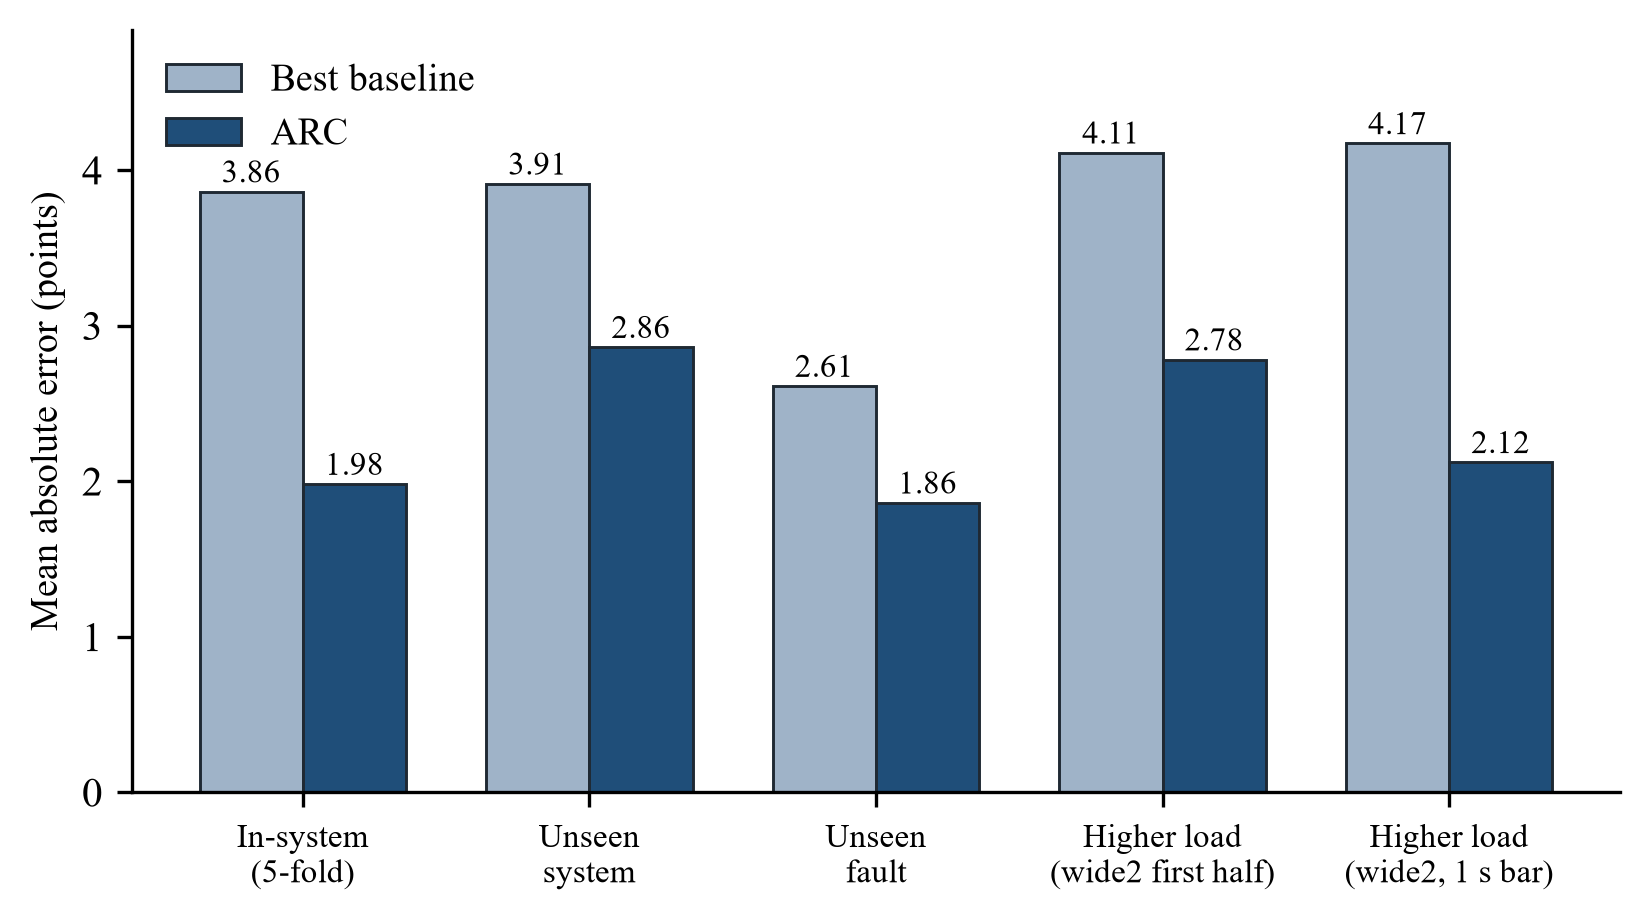
\includegraphics[width=0.92\textwidth]{results.png}
\caption{ARC against the best baseline in five tests.}
\label{fig:results}
\end{figure}

ARC identifies the most damaged service in 78\% of incidents, against 40\% for trees. The trees, however, rank all services better (Spearman correlation 0.75 against 0.68), so ARC does not win on every metric. For harmed-or-not classification ARC reaches an F1 score of 0.77 against 0.75 for the classifier. Across latency bars from 50~ms to 1~s, ARC's error is 0.21 to 0.56 times the error of predicting no damage. On the batch-1 test split alone, ARC's error is 1.83 against 6.46 for the dependency map and 9.03 for the runbook average.

\subsection{Held-out faults and the noise floor}
Table~\ref{tab:held} and Figure~\ref{fig:held} show ARC on 147 episodes of fault types that were not in the training data. ARC is accurate on call cuts and no-fault episodes, but the average is dominated by the four-times traffic surge (error 22.16), a fault of a new kind with no failing component, which the model does not predict. Over all held-out episodes the error is 7.57, level with the best baseline (role rule, 7.51) and below predicting no damage (9.21).

\begin{table}[H]
\centering
\caption{ARC on conditions never seen in training.}
\label{tab:held}
\small
\begin{tabular}{@{}lccc@{}}
\toprule
Condition & Episodes & ARC error & Worst service hit (share bad) \\
\midrule
call cut ts-assurance-service & 21 & 0.98 & 36\% \\
call cut ts-config-service & 21 & 4.65 & 67\% \\
call cut ts-order-other-service & 21 & 3.24 & 40\% \\
traffic surge 3x & 21 & 6.09 & 33\% \\
traffic surge 4x & 21 & 22.16 & 40\% \\
no fault & 21 & 3.20 & 44\% \\
pod-kill & 21 & 5.51 & 41\% \\
\textbf{all held-out} & \textbf{147} & \textbf{7.57} & \textbf{42\%} \\
\bottomrule
\end{tabular}
\end{table}

\begin{figure}[H]
\centering
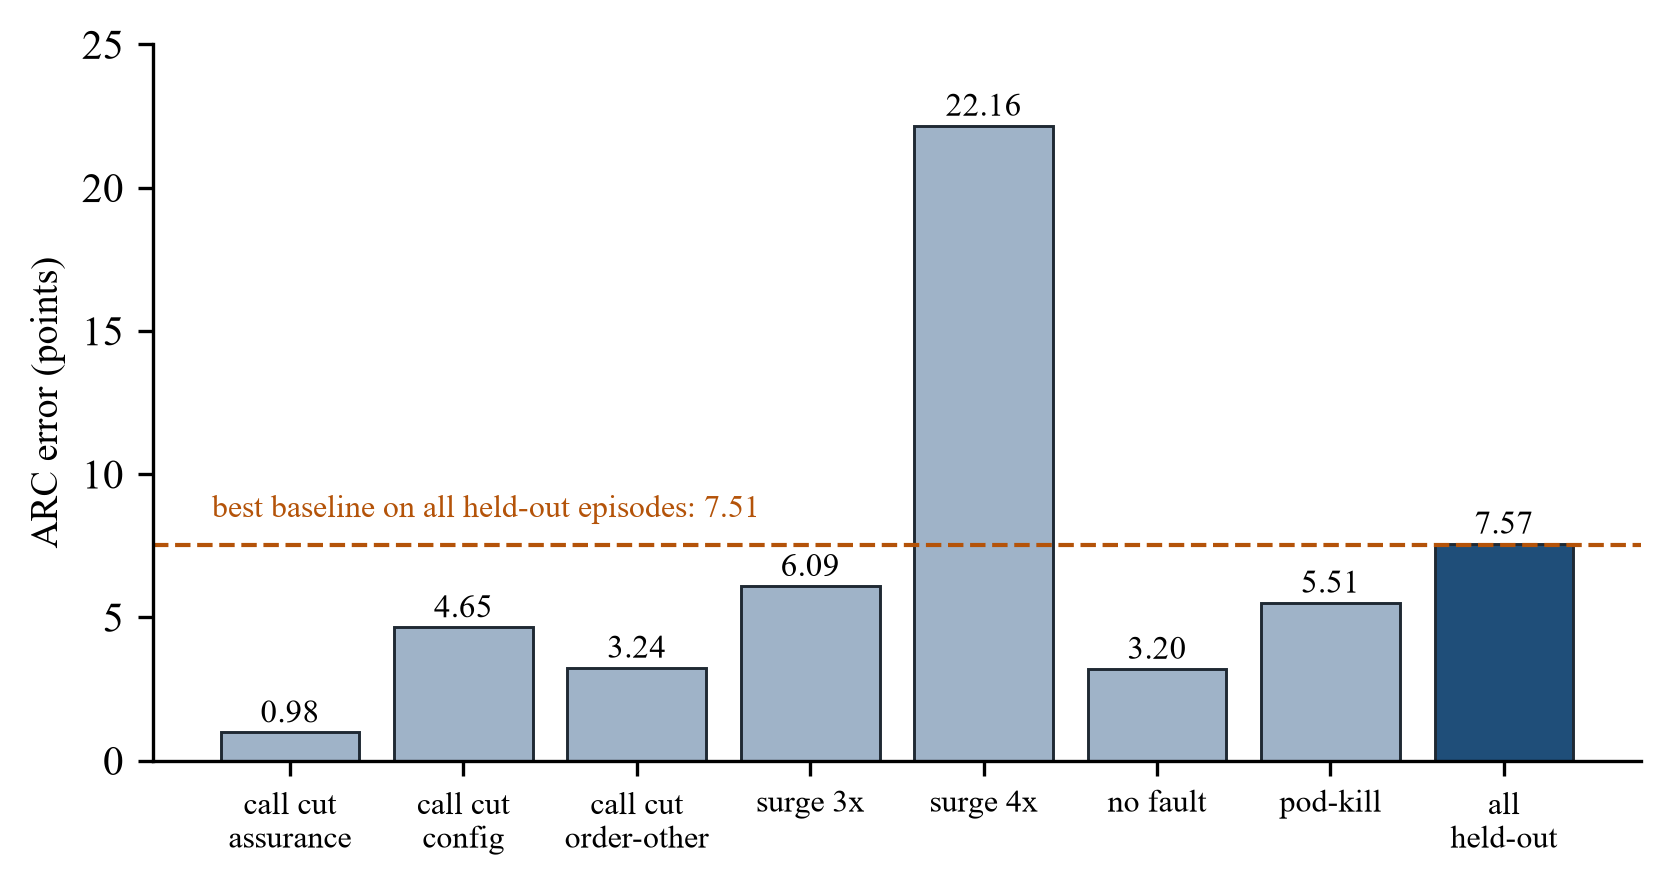
\includegraphics[width=0.92\textwidth]{heldout.png}
\caption{ARC error on conditions never seen in training.}
\label{fig:held}
\end{figure}

The same incident repeated five times does not give the same numbers: total damage varies by 12 to 27\%. No predictor can therefore score below 3.08 points on these incidents; ARC is 2.1 points above this floor and the trees are 7.2 points above it.

\subsection{Uncertainty, speed and decisions}
\textbf{Uncertainty.} When the five model copies disagree the prediction is more often wrong. In the 20\% of episodes with the highest disagreement the error is 3.7 against 1.3 (in-system), 7.2 against 2.0 (unseen system) and 4.5 against 1.2 (unseen fault).

\noindent\textbf{Speed.} The model scores one action in 4~ms and all six in about 25~ms; the full tool takes about 350~ms before optimisation. The LLM judge needs 3.6~s and is no better than predicting no damage.

\noindent\textbf{Explanation, ranking and gate.} The blast-radius explanation reaches a hit-set F1 of 0.74, against 0.64 for a dependency map. Ranking the six actions by predicted net damage puts 86\% of action pairs in the right order, against 80\% for a runbook-style average. The gate blocks 1.6\% of safe actions and detects 84\% of harmful ones.

\section{Validation and Known Limits of the Data}
\textbf{What has been checked.} (i) The latency bar was fitted on healthy episodes only and checked on healthy episodes that were not used to fit it (Train Ticket: fitted on 12, checked on 8). (ii) Labels are reported at three bars, so the results do not depend on one threshold. (iii) Repeating the same incident gives the measurement noise (12 to 27\%, floor 3.08). (iv) Plans, discard rules and scoring rules were fixed before the runs and are applied by code. (v) Every released file has a checksum, the archives pass a gzip test, the loader returns the expected counts for every split, and a scan found no host names or user paths in the released files.

\noindent\textbf{Known issues.} The datasheet lists them; the ones that change results are:
\begin{enumerate}
\item \textbf{Saturation.} In 389 of 1,795 episodes users were already at least 80\% bad before the action. They are flagged and should be excluded, or the 1~s bar used, when ranking actions.
\item \textbf{Drift in wide2.} Two tables read by the cancel flow were not cleaned, so the cancel flow slowed from 77 to 131~ms during wide2. Labels after block 24 are inflated for that flow; the first half of wide2 or the 1~s bar should be used.
\item \textbf{One system, one machine, one copy per service.} Fault levels were dosed on this machine and are not a measure of severity.
\item \textbf{Short bursts are invisible.} The label averages over 180~s; a burst of a few seconds stays in the raw requests only.
\end{enumerate}

\noindent\textbf{What has not been done yet.} The labels measure what the users see (the share of bad requests); no operator has judged whether a given rise matters. All data of version 1.0 was recorded on one machine with one pipeline, so independent replication is still open. Further validity tests (dose--response of the fault levels, agreement of the service-side counters with the load generator's own log, and a check of damage against the call graph) are planned.

\section{Second Application: Online Boutique}
To test whether the pipeline works beyond one application, the testbed was ported to Online Boutique, a Google demonstration shop of 11 services and a cache. The port needed several changes. Three services (ad, cart and shipping) are written in Go, C\# and Java and emit no server-side spans, so they are named through the service graph from their callers' client spans and their labels are computed from the callers' view of the calls (caller view, threshold 100~ms). Draining a service is done with a Chaos Mesh network partition because Online Boutique has no service registry. A restart whose effect lasts about 10~s is invisible in a 180~s label. The latency bar was calibrated at 8 requests per second on healthy episodes (0 false harms in 42 held-out service verdicts, and every service receives a verdict).

A campaign of 280 episodes (40 blocks of 7, eight fault conditions, six actions) was planned in advance. \todo{At the time of writing about 200 of the 280 planned episodes were recorded; insert the final counts before submission.} Two harness faults were found by the safety rules and fixed during the run: a failed drain left its network partition behind, and a CPU squeeze that was followed by a scale-up left a pod throttled; five episodes affected by the second fault are kept but excluded. Saturation in this campaign (about 21\% of episodes) comes only from network delay and hung pods, which is a finding about those faults; packet loss, CPU squeeze, pod-kill and no-fault episodes were never saturated. The no-op control is clean (5 harm rows of 618 service rows), and drain is the most harmful action, as expected. The Online Boutique results are therefore treated as a replication with stated limits, and Train Ticket remains the main benchmark.

% ----------------------------------------------------------------
\chapter{Conclusion}
\section{Conclusion}
Automated remediation tools decide whether to act from their confidence in a diagnosis, and nothing tells them what the action will cost the services around its target. ARC fills this gap. We built a repeatable testbed, recorded 1,795 controlled incidents on the Train Ticket application with all six remediation actions applied to each fault condition, and labelled each service by the rise in its share of failed or slow requests, computed from exact request counters. A three-layer graph network over the call graph, combined with a tree model, predicts this damage before the action is applied.

The model cuts the prediction error roughly in half against the best baseline in every test: 1.98 against 3.86 percentage points on new incidents, 2.86 against 3.91 on an unseen system, 1.86 against 2.61 on an unseen fault, and 2.78 against 4.11 at twice the load. It names the most damaged service in 78\% of incidents, ranks 86\% of action pairs correctly, explains the blast radius with a hit-set F1 of 0.74, and drives a gate that blocks 1.6\% of safe actions and detects 84\% of harmful ones. Scoring all six actions takes about 25~ms, so an agent can ask before every action. The disagreement of the five model copies is a useful warning: the episodes with the highest disagreement have several times the error.

The dataset, with raw telemetry, labels, splits, a datasheet and a loader, is prepared for open release, and a second application, Online Boutique, has been used to test whether the pipeline carries over.

\section{Limitations}
\begin{itemize}
\item The evaluation covers one main application on one machine, with one copy of each service. A second application is under evaluation and is a replication with stated limits.
\item Generalisation to new kinds of incident is still weak: over all held-out episodes the error (7.57) is level with the best baseline (7.51), and it reaches 22.16 under a four-times traffic surge, which has no failing component.
\item The trees rank all services better than ARC (Spearman 0.75 against 0.68), and some action rankings change with the latency bar.
\item Labels average over 180~s, so bursts of a few seconds are not seen, and labels measure what users see, not whether an operator would consider the rise important.
\item Saturated episodes (389 of 1,795) and the drift in the second half of wide2 need care when the data is reused.
\end{itemize}

\section{Future Work}
\begin{itemize}
\item \textbf{Model:} use temporal telemetry, the age of the fault, the number of replicas and traffic changes as inputs; evaluate calibrated uncertainty intervals (conformal prediction~[25],[26]); predict the distribution of latency rather than a single share.
\item \textbf{Integration:} connect ARC to a root-cause diagnosis agent and to a remediation executor; optimise the complete tool toward a latency below 50~ms; monitor baseline drift.
\item \textbf{Data and evaluation:} finish the Online Boutique campaign and release it as version 1.1; run the planned validity tests (dose--response, agreement of independent measurements, call-graph mechanism); test the gate with an agent benchmark such as AIOpsLab [9]; release the dataset on Zenodo and Hugging Face.
\end{itemize}

% ----------------------------------------------------------------
\begin{thebibliography}{99}
\addcontentsline{toc}{chapter}{References}
\setlength{\itemsep}{2pt}
\small
\bibitem{r1} C. Dai, Z. Yan, C. Lei, Q. Li, L. Zhang, ``Safe Remediation as Risk-Constrained Intervention Decision in Microservice Systems,'' arXiv:2607.20005, 2026.
\bibitem{r2} W. Cai et al., ``Can AI Remediate Backend Failures Safely? GuardedAct with Blast-Radius-Aware Sandboxing,'' arXiv:2609.11264, 2026.
\bibitem{r3} L. Bindschaedler, ``Rebooting Microreboot: Architectural Support for Safe, Parallel Recovery in Microservice Systems,'' Proc. ARCS, 2026. arXiv:2604.09963.
\bibitem{r4} L. Zhang et al., ``MicroRemed: Benchmarking LLMs in Microservices Remediation,'' arXiv:2511.01166, 2025.
\bibitem{r5} L. Zhang et al., ``E2E-REME: Towards End-to-End Microservices Auto-Remediation via Experience-Simulation Reinforcement Fine-Tuning,'' FSE 2026. arXiv:2604.11094.
\bibitem{r6} A. Malik, ``Autonomous Incident Resolution at Hyperscale: An Agentic AI Architecture for Network Operations,'' arXiv:2606.09122, 2026.
\bibitem{r7} J. Qi et al., ``Can LLMs Really Recover Microservice Failures? A Recovery-Aware Evaluation of Diagnosis-to-Action Reasoning,'' arXiv:2607.04623, 2026.
\bibitem{r8} S. Fatima et al., ``CRRL: A Causality-Based Reinforcement Learning Framework for Autonomous System Recovery,'' arXiv:2607.03177, 2026.
\bibitem{r9} Y. Chen et al., ``AIOpsLab: A Holistic Framework to Evaluate AI Agents for Enabling Autonomous Clouds,'' arXiv:2501.06706, 2025.
\bibitem{r10} J. Clark et al., ``SREGym: A Live Benchmark for AI SRE Agents with High-Fidelity Failure Scenarios,'' arXiv:2605.07161, 2026.
\bibitem{r11} Y. Chen et al., ``STRATUS: A Multi-agent System for Autonomous Reliability Engineering of Modern Clouds,'' arXiv:2506.02009, 2025.
\bibitem{r12} X. Zhang, Q. Wang, M. Li, Y. Yuan, M. Xiao, F. Zhuang, D. Yu, ``TAMO: Fine-Grained Root Cause Analysis via Tool-Assisted LLM Agent with Multi-Modality Observation Data in Cloud-Native Systems,'' IEEE Trans. Services Computing, 2025. arXiv:2504.20462.
\bibitem{r13} L. Pham, H. Zhang, H. Ha, F. Salim, X. Zhang, ``RCAEval: A Benchmark for Root Cause Analysis of Microservice Systems with Telemetry Data,'' arXiv:2412.17015, 2024.
\bibitem{r14} A. Fang et al., ``Rethinking the Evaluation of Microservice RCA with a Fault Propagation-Aware Benchmark,'' FSE 2026. arXiv:2510.04711.
\bibitem{r15} F. Gao et al., ``Are GNNs Actually Effective for Multimodal Fault Diagnosis in Microservice Systems?,'' arXiv:2501.02766, 2025.
\bibitem{r16} I. Bulji\'{c}, ``Does Graph Structure Earn Its Place in Microservice Root-Cause Analysis? A Controlled Study on RCAEval,'' arXiv:2609.27069, 2026.
\bibitem{r17} Y. Gan et al., ``Sage: Leveraging ML to Diagnose Unpredictable Performance in Cloud Microservices,'' arXiv:2112.06263, 2021.
\bibitem{r18} S. Zhang et al., ``Failure Diagnosis in Microservice Systems: A Comprehensive Survey and Analysis,'' arXiv:2407.01710, 2024.
\bibitem{r19} L. Nagalapatti et al., ``Robust Root Cause Diagnosis using In-Distribution Interventions,'' ICLR 2025. arXiv:2505.00930.
\bibitem{r20} X. Zhou et al., ``Fault Analysis and Debugging of Microservice Systems: Industrial Survey, Benchmark System, and Empirical Study,'' IEEE Trans. Software Eng., vol. 47, no. 2, pp. 243--260, 2021 (Train Ticket).
\bibitem{r21} A. Basiri et al., ``Automating Chaos Experiments in Production,'' ICSE-SEIP, 2019. arXiv:1905.04648.
\bibitem{r22} Chaos Mesh, a cloud-native chaos engineering platform for Kubernetes, \url{https://chaos-mesh.org}.
\bibitem{r23} S. Smith et al., ``Benchmarks for End-to-End Microservices Testing,'' IEEE SOSE, 2023. arXiv:2306.05895.
\bibitem{r24} Y. Feng et al., ``CORA: Conformal Risk-Controlled Agents for Safeguarded Mobile GUI Automation,'' arXiv:2604.09155, 2026.
\bibitem{r25} J. Lekeufack, A. N. Angelopoulos, A. Bajcsy, M. I. Jordan, J. Malik, ``Conformal Decision Theory: Safe Autonomous Decisions from Imperfect Predictions,'' ICRA 2024. arXiv:2310.05921.
\bibitem{r26} A. N. Angelopoulos, S. Bates, ``A Gentle Introduction to Conformal Prediction and Distribution-Free Uncertainty Quantification,'' arXiv:2107.07511, 2021.
\end{thebibliography}

\end{document}

